\documentclass{article}
\usepackage{graphicx}
\usepackage{multirow}% Required for multirows
\usepackage{siunitx} % Required for alignment
\sisetup{
round-mode  = places, %Rounds numbers
round-precision  = 2, % to 2 places
}
\begin{document}
	\begin{table}[h!]
		\begin{center}
			\caption{Multirow table.}
			\label{tab:table1}
			\begin{tabular}{l|S|r}
				\hline
				\textbf{Value 1} & \textbf{Value 2} & \textbf{Value 3}\\
				$\alpha$ & $\beta$ & $\gamma$ \\
				\hline
				\multirow{2}{*}{12} & 1110.1 & a\\ % <-- Combining 2 rows with arbitrary with (*) and content 12
				& 10.1 & b\\ % <-- Content of first column omitted.
				\hline
				14 & 25.113231 &
				\multirow{2}{*}{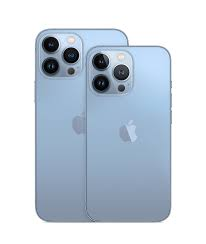
\includegraphics[width=0.05\linewidth]{iphone13}}\\
				25 & 345.113231 & \\
				\hline
				36 & 35.123531 & c \\
				\hline
			\end{tabular}
		\end{center}
	\end{table}
\end{document}